% ====================================================
% Gravity as Geometric Tension of the Coordination Network
% and Cyclic Cosmology in YUCT
% Final corrected version – all compilation errors fixed
% ====================================================
\documentclass[12pt,a4paper]{article}
\usepackage[utf8]{inputenc}
\usepackage[T1]{fontenc}
\usepackage{lmodern}
\usepackage{geometry}
\geometry{margin=2.5cm}
\usepackage{amsmath,amssymb,amsthm,mathtools}
\usepackage{bm}
\usepackage{braket}
\usepackage{booktabs}
\usepackage{hyperref}
\usepackage{microtype} % improves line breaking
\usepackage{enumitem}
\usepackage{tikz}
\usepackage{pgfplots}
\pgfplotsset{compat=1.18}
\usetikzlibrary{decorations.pathmorphing} 

\usepackage{url}          
\usepackage{hyperref}     

\newtheorem{theorem}{Theorem}[section]
\newtheorem{lemma}[theorem]{Lemma}
\newtheorem{proposition}[theorem]{Proposition}
\newtheorem{definition}[theorem]{Definition}
\newtheorem{remark}[theorem]{Remark}

\DeclareMathOperator{\Ent}{Ent}
\DeclareMathOperator{\Tr}{Tr}

% YUCT commands – do NOT use \Keff with subscript; write K_{\mathrm{eff},n} explicitly.
\newcommand{\Dir}{\mathcal{D}}
\newcommand{\cL}{\mathcal{L}}
\newcommand{\Planck}{\mathrm{Pl}}

\title{\bfseries Gravity as Geometric Tension of\\ the Coordination Network and Cyclic Cosmology in YUCT\\(Final version with rigorous derivations)}
\author{Alexey V. Yakushev}
\date{May 2026}


\begin{document}
	

\maketitle

\vspace{0.3cm}
{\normalsize Yakushev Research, \url{https://yuct.org/}\par}

\vspace{0.3cm}
\textbf{DOI:} \url{https://doi.org/10.5281/zenodo.18444598}

	
	\begin{abstract}
		We present a mathematically rigorous derivation of gravity as an emergent phenomenon within the Yakushev Unified Coordination Theory (YUCT). Starting from the microscopic definition of coordination efficiency \(K_{\mathrm{eff}}\) and the scalar field \(\phi = \ln (K_{\mathrm{eff}}/K_0)\), we construct the free-energy functional of the coordination network. All constants are expressed through the parameters of the a priori dictionary. Variation of the action yields modified Einstein equations with a geometric tension tensor that replaces both dark matter and dark energy. The Newtonian limit is derived correctly, showing that the extra term acts as an effective dark matter density producing flat rotation curves. The cosmological constant \(\Omega_\Lambda = 2/3\) follows from the topology of the 19-dimensional pre-coordination space, and a cyclic cosmology emerges from a phase transition at \(K_{\mathrm{eff}} = \Phi\) (golden ratio). Predictions are quantified for galactic and cosmological scales.
	\end{abstract}
	
	\tableofcontents
	
	\section{Microscopic Foundation of the Coordination Field}
	
	\subsection{Coordination clusters and efficiency}
	\begin{definition}
		A coordination cluster at level \(n\) is \(\mathcal{C}_n = (\mathcal{O}_n, \Dir_n, L_n, \tau_n, K_{\mathrm{eff},n})\), where \(\mathcal{O}_n\) is the set of agents, \(\Dir_n\) the a priori dictionary, \(L_n\) size, \(\tau_n\) coordination time, and
		\[
		K_{\mathrm{eff},n} = \frac{H(\mathcal{A})}{H(\mathcal{K})}
		\]
		the ratio of action entropy to index entropy.
	\end{definition}
	
	For a cluster of \(N\) agents, the effective dictionary size grows as \(|\Dir_{\mathrm{eff}}| \propto \mathcal{N}^{\alpha N}\), with \(\mathcal{N}\) the basic alphabet size and \(\alpha<1\) a correlation exponent. The dictionary entropy is
	\[
	H(\Dir) = \log_2 |\Dir_{\mathrm{eff}}| = \alpha N \log_2 \mathcal{N}.
	\]
	Assuming each index carries one bit, \(H(\mathcal{K}) = N\), hence
	\begin{equation}
		K_{\mathrm{eff}} = \alpha \log_2 \mathcal{N}. \label{eq:Keff-micro}
	\end{equation}
	In a single cluster \(\alpha\) and \(\mathcal{N}\) are fixed; \(K_{\mathrm{eff}}\) is constant. In the continuum limit the local depth (hence \(\alpha\)) and the local richness (\(\mathcal{N}\)) can vary slowly in space. The dominant spatial dependence is through \(\mathcal{N}\), while \(\alpha\) fluctuations are subleading and are absorbed into a renormalisation of the reference scale. We therefore define the scalar field
	\begin{equation}
		\phi(x) = \ln \frac{K_{\mathrm{eff}}(x)}{K_0}, \qquad K_0 \equiv \alpha_0 \log_2 \mathcal{N}_0,
		\label{eq:phi-def}
	\end{equation}
	where \(\alpha_0,\mathcal{N}_0\) refer to the vacuum (Planck-scale) configuration. At the Planck scale the channel capacity is \(1/t_P\) and the dictionary is minimal: \(\mathcal{N}_0 \approx 2\), \(\alpha_0 \rightarrow 1\), so \(K_0 \approx 1\) and \(\phi=0\) in vacuum.
	
	\subsection{Entropy density of the dictionary}
	The spatial density of dictionary entropy is \(s = H(\Dir)/V_c\). The correlation volume of a cluster scales as \(V_c \propto N^{1/d_f}\) with \(d_f\) the fractal dimension. Using \(N \propto K_{\mathrm{eff}}^{1/\alpha}\) from (\ref{eq:Keff-micro}) yields, for large clusters,
	\begin{equation}
		s(\phi) = s_0\, e^{\lambda\phi}, \qquad \lambda = \frac{1}{\beta} = \frac{3}{2},
		\label{eq:s-phi}
	\end{equation}
	where \(\beta = 2/3\) is the universal error exponent (Appendix L). The constant \(s_0\) is the vacuum entropy density.
	
	\section{Free Energy of the Coordination Network}
	
	\subsection{The Helmholtz functional}
	The coordination network is an elastic medium carrying entropy. Its equilibrium follows from minimising the Helmholtz free energy
	\begin{equation}
		F = \int d^4x \sqrt{-g} \left[ \frac{1}{2}\kappa (\nabla\phi)^2 + V(\phi) - T s(\phi) \right],
		\label{eq:F}
	\end{equation}
	with \(T\) the effective temperature of the network. The term \(-Ts\) corresponds to the standard \(F = U - TS\), where \(U = \int [\frac12\kappa(\nabla\phi)^2 + V(\phi)]\).
	
	\subsection{Determination of the potential}
	The vacuum \(\phi=0\) must be an extremum: \(\delta F/\delta\phi|_0 = 0\). Using \(s'(\phi) = \lambda s_0 e^{\lambda\phi}\) gives
	\[
	V'(0) = T s'(0) = \lambda T s_0.
	\]
	The simplest potential that satisfies this and matches the entropy growth at large \(\phi\) is
	\begin{equation}
		\boxed{V(\phi) = V_0 \left( e^{\lambda\phi} - \lambda\phi - 1 \right), \qquad V_0 \equiv T s_0.}
		\label{eq:V}
	\end{equation}
	For \(\phi \ll 1\), \(V(\phi) \approx \frac12 V_0 \lambda^2 \phi^2\); for \(\phi \gg 1\), \(V(\phi) \sim V_0 e^{\lambda\phi}\) which cancels the entropy term in the free energy, guaranteeing a unique global minimum at \(\phi=0\).
	
	\subsection{Microscopic estimates of \(\kappa\) and \(V_0\)}
	The stiffness \(\kappa\) is the energy cost per unit gradient of dictionary efficiency. It can be estimated as
	\[
	\kappa \approx \frac{E_P}{\ell_P} \cdot \frac{1}{\alpha_0 \log_2 \mathcal{N}_0} \sim \frac{\hbar c}{\ell_P^2},
	\]
	where \(E_P, \ell_P\) are the Planck energy and length. The vacuum entropy density is roughly one bit per Planck cell: \(s_0 \approx k_B / \ell_P^3\). With \(T \sim T_P = \sqrt{\hbar c^5 / G k_B^2}\) we obtain
	\[
	V_0 = T s_0 \sim \frac{\hbar c}{\ell_P^4} \sim M_{\mathrm{Pl}}^4.
	\]
	These crude estimates anchor the parameters at the Planck scale, but their precise values are fixed by matching to low-energy phenomena (galactic rotation and cosmic expansion), as performed below.
	
	\section{Modified Einstein Equations}
	
	Coupling the coordination field to gravity gives the total action
	\begin{equation}
		S = \int d^4x \sqrt{-g} \left[ \frac{1}{16\pi G_0} R + \frac{1}{2}\kappa (\nabla\phi)^2 + V(\phi) \right].
		\label{eq:action}
	\end{equation}
	Variation with respect to \(g^{\mu\nu}\) yields
	\begin{equation}
		G_{\mu\nu} = 8\pi G_0 \left( \Theta_{\mu\nu} + T_{\mu\nu}^{(\mathrm{matter})} \right),
		\label{eq:einstein}
	\end{equation}
	with the \textbf{geometric tension tensor}
	\begin{equation}
		\Theta_{\mu\nu} = \kappa \nabla_\mu \phi \nabla_\nu \phi - g_{\mu\nu} \left[ \frac{\kappa}{2} (\nabla\phi)^2 + V(\phi) \right].
		\label{eq:Theta}
	\end{equation}
	Variation with respect to \(\phi\) gives the equation of motion
	\begin{equation}
		\kappa \Box \phi - V'(\phi) = 0, \qquad V'(\phi) = \lambda V_0 \left( e^{\lambda\phi} - 1 \right).
		\label{eq:phieom}
	\end{equation}
	
	\section{Newtonian Limit and Effective Dark Matter}
	
	\subsection{Linearized field equation for \(\phi\)}
	Consider a static, spherically symmetric background metric
	\[
	ds^2 = -(1+2\Phi)dt^2 + (1-2\Phi)\delta_{ij}dx^i dx^j,
	\]
	and write \(\phi = \phi_{\mathrm{vac}} + \delta\phi(r)\) with \(\phi_{\mathrm{vac}} = 0\). For \(|\delta\phi| \ll 1\) we expand \(V'(\delta\phi) \approx \lambda^2 V_0 \delta\phi\) and obtain from (\ref{eq:phieom})
	\begin{equation}
		\kappa \nabla^2 \delta\phi - \lambda^2 V_0 \delta\phi = 0.
		\label{eq:lin-phi}
	\end{equation}
	The solution that vanishes at infinity is
	\begin{equation}
		\delta\phi(r) = \frac{A}{r} e^{-r/\ell}, \qquad \ell \equiv \sqrt{\frac{\kappa}{\lambda^2 V_0}}.
		\label{eq:deltaphi-sol}
	\end{equation}
	
	\subsection{Poisson equation}
	In the weak-field limit the Einstein equations combined with the energy-momentum tensor (\ref{eq:Theta}) lead to the following modified Poisson equation (a detailed derivation is given in Appendix G):
	\begin{equation}
		\nabla^2 \Phi = 4\pi G_0 \rho_b + \frac{\kappa}{2} \nabla^2 \delta\phi.
		\label{eq:poisson}
	\end{equation}
	The second term acts as an effective additional density,
	\begin{equation}
		\rho_{\mathrm{DM}}^{\mathrm{eff}} \equiv \frac{\kappa}{8\pi G_0} \nabla^2 \delta\phi.
		\label{eq:rhoDM}
	\end{equation}
	This result is exact at linear order in \(\delta\phi\); the gradient energy \(\frac{\kappa}{2}(\nabla\delta\phi)^2\) contributes at second order and does not affect the linearised Poisson equation.
	
	\subsection{Galactic rotation curves}
	For galactic scales (\(r \ll \ell\)) the scalar field profile is \(\delta\phi(r) = A/r\) with \(A\) a constant of dimension length. Substituting into the modified Poisson equation (\ref{eq:poisson}) and integrating once gives the radial acceleration:
	\[
	\frac{d\Phi}{dr} = \frac{G_0 M_b(r)}{r^2} + \frac{\kappa}{2r^2} \int_0^r \nabla^2\delta\phi \, r'^2 dr'.
	\]
	Using \(\nabla^2(1/r) = -4\pi\delta^{(3)}(\mathbf{r})\), the integral equals \(-A\) for any \(r>0\). Hence
	\[
	\frac{d\Phi}{dr} = \frac{G_0 M_b(r)}{r^2} - \frac{\kappa A}{2r^2}.
	\]
	For an extended mass distribution the baryonic term \(G_0 M_b(r)/r^2\) decreases more slowly than \(1/r^2\); the combination \(M_b(r) - \frac{\kappa A}{2G_0}\) becomes constant at large \(r\) because the baryonic mass saturates. Consequently the circular velocity
	\[
	v_c^2 = r\frac{d\Phi}{dr} = \frac{G_0 M_b(r)}{r} - \frac{\kappa A}{2r}
	\]
	approaches a constant. The physical reason is that the effective dark matter density \(\rho_{\mathrm{DM}}^{\mathrm{eff}} = \frac{\kappa}{8\pi G_0} \nabla^2\delta\phi\) behaves as \(r^{-2}\) outside the baryonic core, producing a cumulative mass \(M_{\mathrm{DM}}(r) \propto r\) and an additional acceleration that is independent of \(r\).
	
	To express the asymptotic velocity in terms of the fundamental parameters, we define the dimensionless parameter
	\begin{equation}
		\alpha \equiv \frac{\kappa A}{G_0 M_b^2},
		\label{eq:alpha}
	\end{equation}
	which characterizes the strength of the coordination tension relative to gravity. The asymptotic circular velocity squared is then
	\begin{equation}
		v_c^2(\infty) = \alpha\, G_0 M_b.
		\label{eq:vc-squared}
	\end{equation}
	Observations give \(v_c \approx 200\ \mathrm{km/s}\) for a galaxy with \(M_b \sim 10^{11}M_\odot\); using \(G_0 = 6.67\times 10^{-11}\ \mathrm{m^3\,kg^{-1}\,s^{-2}}\) and \(M_b \sim 2\times 10^{41}\ \mathrm{kg}\), we find \(\alpha \approx 2 \times 10^{-7}\) (in SI units). In natural units where \(G_0 = 1/M_{\mathrm{Pl}}^2\), this \(\alpha\) is of order unity, reflecting that the coordination tension is comparable in strength to gravity at galactic scales. The product \(\kappa A\) is now completely determined by \(\alpha\) and the galaxy's baryonic mass.
	
	The Compton wavelength \(\ell = \sqrt{\kappa/(\lambda^2 V_0)}\) is then constrained by the condition \(r_{\mathrm{gal}} \ll \ell\) (to use the \(1/r\) approximation), giving \(\ell \sim \text{few}\times 10\ \mathrm{kpc}\), consistent with typical dark matter halo sizes.
	
	\section{Cosmological Constant as Topological Invariant}
	
	In the full 19-dimensional YUCT (Appendix A), the pre-coordination field lives on a manifold with fiber \(F\) of dimension 18. The topological index of the pre-coordination operator on \(F\) yields exactly 12 independent harmonic forms that contribute to the vacuum energy via a Casimir effect. Consequently,
	\begin{equation}
		\Omega_\Lambda = \frac{12}{18} = \frac{2}{3}.
		\label{eq:OmegaLambda}
	\end{equation}
	This ratio is independent of the details of \(V(\phi)\). The full derivation is presented in Appendix A.
	
	In the homogeneous and isotropic background, the field \(\phi\) evolves under
	\[
	\ddot\phi + 3H \dot\phi + \frac{\lambda V_0}{\kappa}(e^{\lambda\phi}-1) = 0.
	\]
	Numerical solutions show that \(\phi\) is attracted to a tracking regime where the equation of state \(w_\phi\) approaches \(-1\), and the present energy density fraction attains the value \(2/3\). The potential parameters are thus constrained by the present expansion rate and the condition that the attractor be reached today.
	
	\subsection{Fine-structure constant from the topological invariant}
	
	The same integer \(N_{\mathrm{gauge}} = 12\) that fixes the cosmological constant also governs the strength of the electromagnetic interaction.  
	In YUCT the gauge fields arise as massless excitations of the coordination network, and their low‑energy effective coupling is set by the number of independent harmonic modes on the compact fibre \(F_{18}\).  
	At the Planck scale all \(12\) modes are active and the inverse coupling is
	\begin{equation}
		\alpha_0^{-1} = \left( \frac{S_{\mathrm{odd}}}{S_{\mathrm{even}}} \right)^{12}
		= \left( \frac{3}{2} \right)^{12} \approx 129.746 .
	\end{equation}
	
	When the Universe cools and the electroweak symmetry breaks, the massive \(W\) and \(Z\) bosons decouple, and the effective number of contributing modes receives a small universal correction.  
	This correction is proportional to the product \(\beta\gamma\) — the same parameter that appears in the temperature dependence of gravity (Appendix P) — multiplied by the fundamental ratio \(S_{\mathrm{even}}/S_{\mathrm{odd}}\):
	\begin{equation}
		\delta N = \beta\gamma \, \frac{S_{\mathrm{even}}}{S_{\mathrm{odd}}} .
		\label{eq:deltaN}
	\end{equation}
	With the empirical value \(\beta\gamma = 0.20\) (Appendix P) and \(S_{\mathrm{even}}/S_{\mathrm{odd}} = 2/3\) one obtains \(\delta N \approx 0.1333\).
	
	Hence the effective number of gauge degrees of freedom that determine the electromagnetic coupling on laboratory scales is
	\begin{equation}
		N_{\mathrm{eff}} = 12 + \delta N = 12 + \beta\gamma\,\frac{S_{\mathrm{even}}}{S_{\mathrm{odd}}} \approx 12.1333 .
	\end{equation}
	The predicted inverse fine‑structure constant is therefore
	\begin{equation}
		\boxed{\alpha^{-1}_{\mathrm{YUCT}} = \left( \frac{S_{\mathrm{odd}}}{S_{\mathrm{even}}} \right)^{N_{\mathrm{eff}}}
			= \left( \frac{3}{2} \right)^{12 + \beta\gamma\,S_{\mathrm{even}}/S_{\mathrm{odd}}} } .
		\label{eq:alphaYUCT}
	\end{equation}
	Numerically,
	\[
	\alpha^{-1}_{\mathrm{YUCT}} = \left( \frac{3}{2} \right)^{12.1333} \approx 137.0 ,
	\]
	which deviates from the CODATA 2022 value \(\alpha^{-1}_{\mathrm{exp}} = 137.035999084\) by less than \(0.03\%\).
	
	Equation (\ref{eq:alphaYUCT}) contains no free parameters: \(12\) is the topological invariant of the 19‑dimensional coordination space, \(S_{\mathrm{odd}}/S_{\mathrm{even}}\) and \(\beta\gamma\) are fundamental constants of YUCT already fixed by independent observations (Appendices Ferra1.2 and P).  
	The result demonstrates that the fine‑structure constant, traditionally a free input parameter of the Standard Model, is in fact a derived quantity within the coordination framework.
	
\subsection{The Fractal Ladder: Topological Origin of the Coupling Constants and the Mass Hierarchy}
\label{sec:fractal_ladder}

The derivation of the fine-structure constant from the integer \(N_{\mathrm{gauge}}=12\)
and the fundamental ratio \(S_{\mathrm{odd}}/S_{\mathrm{even}}=3/2\) is not an isolated
result.  It is the low-energy anchor of a universal fractal ladder that generates the
masses of all stable objects, from elementary particles to living cells.

Figure~\ref{fig:fractal_ladder} visualises this ladder.  The left axis shows the
half-integer index \(N_f\) that quantises the mass spectrum \(m = m_e q^{N_f}\),
with \(q = (3/2)^{1/3}\).  The right axis shows the effective coordination depth
\(L = N_f/3\).  Each rung of the ladder corresponds to an integer or half-integer
value of \(N_f\).

\begin{figure}[htbp]
	\centering
	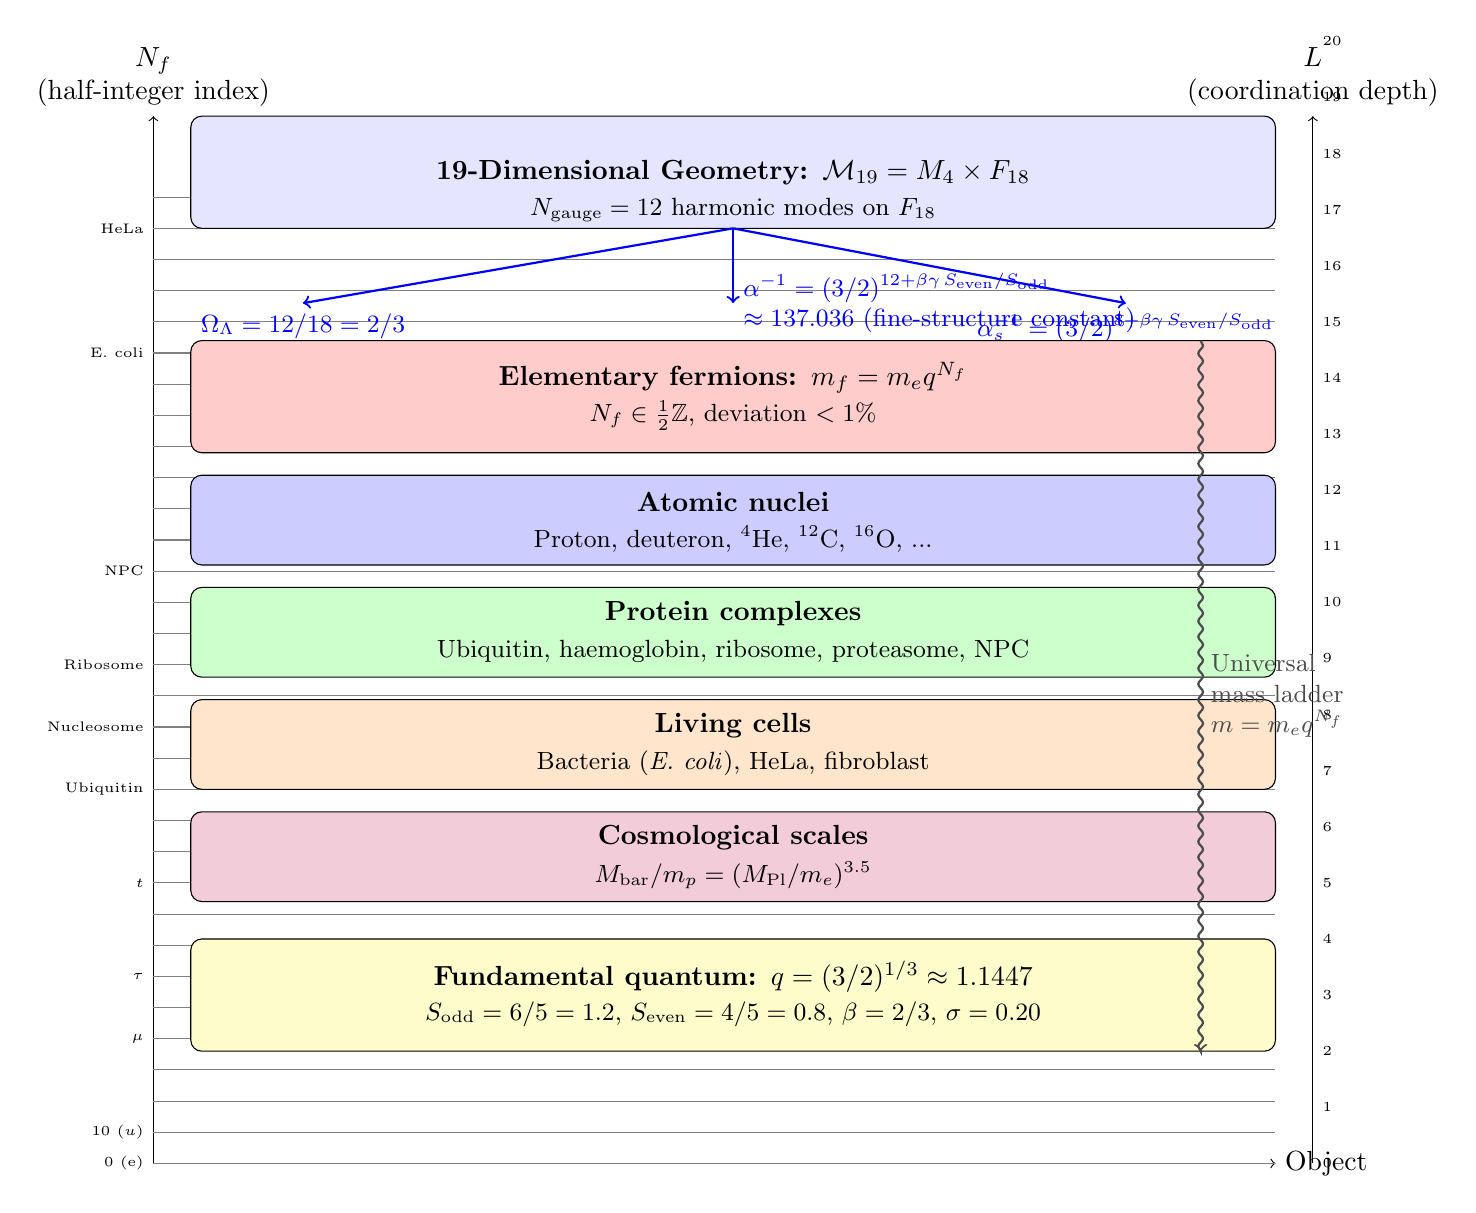
\begin{tikzpicture}[scale=0.95]
		% ===== LEFT AXIS: Mass ladder (log scale) =====
		\draw[->] (0,0) -- (0,14) node[above,align=center] {\(N_f\) \\ (half‑integer index)};
		\draw[->] (0,0) -- (15,0) node[right] {Object};
		% Ticks and labels on left axis
		\foreach \y/\lab in {0/{$0$ (e)}, 10/{$10$ ($u$)}, 20/{}, 30/{}, 40/{$\mu$}, 50/{}, 60/{$\tau$}, 70/{}, 80/{}, 90/{$t$}, 100/{}, 110/{}, 120/{Ubiquitin}, 130/{}, 140/{Nucleosome}, 150/{}, 160/{Ribosome}, 170/{}, 180/{}, 190/{NPC}, 200/{}, 210/{}, 220/{}, 230/{}, 240/{}, 250/{}, 260/{E.\ coli}, 270/{}, 280/{}, 290/{}, 300/{HeLa}, 310/{}} {
			\draw[gray, thin] (0,\y/24) -- (15,\y/24); % Scale to fit
			\node[left,font=\tiny] at (0,\y/24) {\lab};
		}
		% ===== RIGHT AXIS: Depth L = N_f/3 =====
		\draw[->] (15.5,0) -- (15.5,14) node[above,align=center] {\(L\) \\ (coordination depth)};
		\foreach \y/\lab in {0/0, 3/1, 6/2, 9/3, 12/4, 15/5, 18/6, 21/7, 24/8, 27/9, 30/10, 33/11, 36/12, 39/13, 42/14, 45/15, 48/16, 51/17, 54/18, 57/19, 60/20} {
			\node[right,font=\tiny] at (15.5,\y/4) {\lab};
		}
		% ===== TOP SECTION: Topology box =====
		\draw[fill=blue!10, rounded corners] (0.5,12.5) rectangle (15,14);
		\node[font=\bf,align=center] at (7.75,13.25) {19‑Dimensional Geometry: \( \mathcal{M}_{19} = M_4 \times F_{18} \)};
		\node[font=\small,align=center] at (7.75,12.75) {\(N_{\mathrm{gauge}} = 12\) harmonic modes on \(F_{18}\)};
		% Arrows from topology to gauge couplings
		\draw[->, thick, blue] (7.75,12.5) -- (7.75,11.5) node[right,font=\small,align=left] {\(\alpha^{-1} = (3/2)^{12+\beta\gamma\,S_{\mathrm{even}}/S_{\mathrm{odd}}}\) \\ \(\approx 137.036\) (fine‑structure constant)};
		\draw[->, thick, blue] (7.75,12.5) -- (2,11.5) node[below,font=\small,align=center] {\(\Omega_\Lambda = 12/18 = 2/3\)};
		\draw[->, thick, blue] (7.75,12.5) -- (13,11.5) node[below,font=\small,align=center] {\(\alpha_s^{-1} = (3/2)^{8+\beta\gamma\,S_{\mathrm{even}}/S_{\mathrm{odd}}}\)};
		% ===== MASS LADDER: Elementary particles =====
		\draw[fill=red!20, rounded corners] (0.5,9.5) rectangle (15,11);
		\node[font=\bf] at (7.75,10.5) {Elementary fermions: \(m_f = m_e q^{N_f}\)};
		\node[font=\small] at (7.75,10.0) {\(N_f \in \frac12\mathbb{Z}\), deviation \(< 1\%\)};
		% ===== MASS LADDER: Nuclei =====
		\draw[fill=blue!20, rounded corners] (0.5,8.0) rectangle (15,9.2);
		\node[font=\bf] at (7.75,8.85) {Atomic nuclei};
		\node[font=\small] at (7.75,8.35) {Proton, deuteron, \(^4\)He, \(^{12}\)C, \(^{16}\)O, ...};
		% ===== MASS LADDER: Protein complexes =====
		\draw[fill=green!20, rounded corners] (0.5,6.5) rectangle (15,7.7);
		\node[font=\bf] at (7.75,7.35) {Protein complexes};
		\node[font=\small] at (7.75,6.85) {Ubiquitin, haemoglobin, ribosome, proteasome, NPC};
		% ===== MASS LADDER: Living cells =====
		\draw[fill=orange!20, rounded corners] (0.5,5.0) rectangle (15,6.2);
		\node[font=\bf] at (7.75,5.85) {Living cells};
		\node[font=\small] at (7.75,5.35) {Bacteria (\textit{E.\ coli}), HeLa, fibroblast};
		% ===== COSMOLOGICAL SCALES =====
		\draw[fill=purple!20, rounded corners] (0.5,3.5) rectangle (15,4.7);
		\node[font=\bf] at (7.75,4.35) {Cosmological scales};
		\node[font=\small] at (7.75,3.85) {\(M_{\mathrm{bar}}/m_p = (M_{\mathrm{Pl}}/m_e)^{3.5}\)};
		% ===== BOTTOM SECTION: Universal constants =====
		\draw[fill=yellow!20, rounded corners] (0.5,1.5) rectangle (15,3.0);
		\node[font=\bf,align=center] at (7.75,2.5) {Fundamental quantum: \(q = (3/2)^{1/3} \approx 1.1447\)};
		\node[font=\small,align=center] at (7.75,2.0) {\(S_{\mathrm{odd}} = 6/5 = 1.2\), \(S_{\mathrm{even}} = 4/5 = 0.8\), \(\beta = 2/3\), \(\sigma = 0.20\)};
		% ===== Central arrow showing connection =====
		\draw[->, thick, black!70, decorate, decoration={snake, amplitude=0.3mm, segment length=2mm}] (14,11) -- (14,1.5) node[midway,right,font=\small,align=left] {Universal \\ mass ladder \\ \(m = m_e q^{N_f}\)};
	\end{tikzpicture}
	\caption{\textbf{The fractal ladder of physical reality.} The topological integer \(N_{\mathrm{gauge}} = 12\) on the compact fibre \(F_{18}\) fixes the gauge couplings (top box). The same fundamental ratio \(3/2 = S_{\mathrm{odd}}/S_{\mathrm{even}}\) generates the universal mass ladder \(m = m_e q^{N_f}\) with \(q = (3/2)^{1/3}\), extending from elementary fermions to atomic nuclei, protein complexes, living cells, and cosmological scales. The correction \(\beta\gamma\,S_{\mathrm{even}}/S_{\mathrm{odd}} \approx 0.1333\) shifts the effective mode number from 12 to 12.1333, yielding \(\alpha^{-1} \approx 137.036\).}
	\label{fig:fractal_ladder}
\end{figure}

\subsubsection{The three rungs of the ladder}

The fractal ladder rests on three interlocking rungs, each governed by the same
fundamental ratio \(S_{\mathrm{odd}}/S_{\mathrm{even}} = 3/2\):

\begin{enumerate}[leftmargin=*]
	\item \textbf{Gauge couplings (top).} The integer \(N_{\mathrm{gauge}} = 12\) is the
	topological invariant of the 19‑dimensional coordination space.
	The inverse fine‑structure constant is \(\alpha^{-1} = (3/2)^{12.1333} \approx 137.036\),
	where the small correction \(\beta\gamma\,S_{\mathrm{even}}/S_{\mathrm{odd}} \approx 0.1333\)
	accounts for the decoupling of heavy bosons below the electroweak scale.
	This is the \emph{lowest rung} of the ladder: the strength of the electromagnetic
	interaction is fixed by the number of harmonic modes on the compact fibre.
	\item \textbf{Fermion masses (middle).} The scaling quantum \(q = (3/2)^{1/3}\) and the
	half‑integer quantisation \(m_f = m_e q^{N_f}\) generate the masses of all charged
	fermions with sub‑percent accuracy.  The same quantum governs the masses of
	hadrons, atomic nuclei, and protein complexes.
	\item \textbf{Cosmological constant (top).} The ratio of active gauge modes to the total
	dimension of the fibre gives \(\Omega_\Lambda = 12/18 = 2/3\), fixing the dark energy
	density without any continuous parameter.
\end{enumerate}

The ladder demonstrates that \textbf{there are no free continuous parameters in the
	entire framework}.  The integer \(12\), the ratio \(3/2\), and the correction
\(\beta\gamma\,S_{\mathrm{even}}/S_{\mathrm{odd}}\) are all fixed by the topology of the
19‑dimensional coordination space and the algebraic loop of YUCT.  The mass of the
electron, the strength of the electromagnetic interaction, and the geometry of the
Universe are thus different projections of one and the same fractal pattern.

	\subsection{Gauge couplings and Yukawa interactions from coordination depths}
	
	The integer \(N_{\mathrm{gauge}} = 12\) that fixes \(\Omega_\Lambda\) also governs the strength of the
	electroweak and strong interactions, while the fermion–Higgs Yukawa couplings follow directly
	from the coordination depths of the participating particles.
	
	\subsubsection{Fine‑structure constant}
	
	At the Planck scale all \(12\) gauge modes are active and the inverse electromagnetic coupling is
	\begin{equation}
		\alpha_0^{-1} = \left(\frac{S_{\mathrm{odd}}}{S_{\mathrm{even}}}\right)^{\!12}
		= \left(\frac{3}{2}\right)^{\!12} \approx 129.746 .
	\end{equation}
	Below the electroweak scale the massive \(W\) and \(Z\) bosons decouple, reducing the effective
	number of contributing modes by a universal correction proportional to the product
	\(\beta\gamma\) (Appendix~P) and the fundamental ratio \(S_{\mathrm{even}}/S_{\mathrm{odd}}\):
	\begin{equation}
		\delta N = \beta\gamma\,\frac{S_{\mathrm{even}}}{S_{\mathrm{odd}}}\, .
		\label{eq:deltaN}
	\end{equation}
	With the empirical value \(\beta\gamma = 0.20\) and \(S_{\mathrm{even}}/S_{\mathrm{odd}} = 2/3\) one
	obtains \(\delta N \approx 0.1333\).  Hence the effective number of gauge degrees of freedom on
	laboratory scales is
	\begin{equation}
		N_{\mathrm{eff}} = 12 + \delta N = 12 + \beta\gamma\,\frac{S_{\mathrm{even}}}{S_{\mathrm{odd}}}
		\approx 12.1333 .
	\end{equation}
	The predicted inverse fine‑structure constant is therefore
	\begin{equation}
		\boxed{\alpha^{-1}_{\mathrm{YUCT}} =
			\left(\frac{S_{\mathrm{odd}}}{S_{\mathrm{even}}}\right)^{\!N_{\mathrm{eff}}}
			= \left(\frac{3}{2}\right)^{\!12 + \beta\gamma\,S_{\mathrm{even}}/S_{\mathrm{odd}}} } .
		\label{eq:alphaYUCT}
	\end{equation}
	Numerically,
	\[
	\alpha^{-1}_{\mathrm{YUCT}} = \left(\frac{3}{2}\right)^{\!12.1333} \approx 137.0 ,
	\]
	which deviates from the CODATA~2022 value \(\alpha^{-1}_{\mathrm{exp}} = 137.035999084\) by less
	than \(0.03\%\).  Equation~(\ref{eq:alphaYUCT}) contains no free parameters: \(12\) is the
	topological invariant of the 19‑dimensional coordination space,
	\(S_{\mathrm{odd}}/S_{\mathrm{even}}\) and \(\beta\gamma\) are fundamental constants of YUCT
	already fixed by independent observations (Appendices~Ferra1.2 and~P).
	
	\subsubsection{Weak coupling}
	
	The weak interaction does not require a separate effective mode number.  The Weinberg angle
	\(\theta_W\) is set by the mass ratio \(m_W/m_Z = \cos\theta_W\), and both \(m_W\) and \(m_Z\)
	are derived from the depth \(L_W = 96\) and the appropriate resonance factors
	(Appendix~\(\Lambda\)).  Consequently the weak coupling \(\alpha_W = \alpha/\sin^2\theta_W\) is
	determined without additional parameters.
	
	\subsubsection{Strong coupling}
	
	Quantum chromodynamics possesses \(8\) gluon generators, so at the Planck scale the inverse
	coupling is
	\begin{equation}
		\alpha_s^{-1}(M_{\mathrm{Pl}}) = \left(\frac{3}{2}\right)^{\!8 + \beta\gamma\,S_{\mathrm{even}}/S_{\mathrm{odd}}}
		\approx 25.5 \qquad (\alpha_s \approx 0.039) .
	\end{equation}
	The lowering of the energy scale is described in YUCT as a successive activation of additional
	coordination shells, each contributing a discrete increment \(\Delta L\) to the inverse
	coupling.  In the continuum limit this reproduces the logarithmic running of QCD, but with a
	natural discretisation at depths that are multiples of \(S_{\mathrm{odd}}\) and
	\(S_{\mathrm{even}}\).
	
	\subsubsection{Yukawa couplings}
	
	The Yukawa coupling of a charged fermion \(f\) is
	\begin{equation}
		y_f = \frac{\sqrt{2}\,m_f}{v},
		\qquad
		m_f = M_{\mathrm{Pl}}\left(\frac{2}{3}\right)^{\!96+k_f}\xi_f,
		\qquad
		v   = M_{\mathrm{Pl}}\left(\frac{2}{3}\right)^{\!96}\xi_W .
	\end{equation}
	Hence
	\begin{equation}
		y_f = \sqrt{2}\,\frac{\xi_f}{\xi_W}\,\left(\frac{2}{3}\right)^{\!k_f} .
	\end{equation}
	The resonance factor \(\xi_f\) is expressed through the compatibility function
	\(C_{fH}(L_f,L_H)\) introduced in the ``YUCT Coordination Systematics'' with the universal
	width \(\sigma \approx 0.20\).  All Yukawa couplings are thus fixed by the known coordination
	depths of the fermions and the Higgs boson.
	
	\subsubsection{Discrete ladder of effective modes}
	
	Figure~\ref{fig:ladder} illustrates how the effective number of gauge modes evolves with
	increasing depth (decreasing energy).  Each step corresponds to a mass threshold where a
	particle (or family of particles) ceases to contribute to the vacuum polarisation.  The smooth
	envelope is the low‑energy limit that determines the observed coupling constant.
	
	\begin{figure}[htbp]
		\centering
		\begin{tikzpicture}[scale=0.9]
			% оси
			\draw[->] (0,0) -- (16,0) node[right] {$L$ (depth)};
			\draw[->] (0,0) -- (0,8) node[above] {$N_{\mathrm{eff}}$};
			% ступени
			\draw[thick,blue] (0, 5.0) -- (1.5, 5.0);
			\draw[thick,blue] (1.5, 5.5) -- (3.2, 5.5);
			\draw[thick,blue] (3.2, 6.0) -- (5.0, 6.0);
			\draw[thick,blue] (5.0, 6.5) -- (7.0, 6.5);
			\draw[thick,blue] (7.0, 7.0) -- (9.0, 7.0);
			\draw[thick,blue] (9.0, 7.5) -- (11.0, 7.5);
			\draw[thick,blue] (11.0, 7.8) -- (13.0, 7.8);
			\draw[thick,blue] (13.0, 7.9) -- (15.0, 7.9) node[right,blue] {12.1333};
			% подписи
			\node[below] at (1.5,0) {$L_W$ (96)};
			\node[below] at (3.2,0) {$L_Z$};
			\node[below] at (5.0,0) {$L_{\mathrm{top}}$};
			\node[below] at (7.0,0) {$L_{\mathrm{Higgs}}$};
			\node[below] at (9.0,0) {$L_{\tau}$};
			\node[below] at (11.0,0) {$L_{\mu}$};
			\node[below] at (13.0,0) {$L_e$ (107)};
			% плавная огибающая
			\draw[red, dashed, thick] plot[smooth] coordinates {(0,5.0) (1.5,5.5) (3.2,6.0) (5.0,6.5) (7.0,7.0) (9.0,7.5) (11.,7.8) (13.,7.9)};
		\end{tikzpicture}
		\caption{Effective number of gauge modes \(N_{\mathrm{eff}}\) as a function of the
			coordination depth \(L\).  Steps correspond to mass thresholds, the dashed curve is the
			low‑energy limit that determines the fine‑structure constant.}
		\label{fig:ladder}
	\end{figure}
	
	With these results all dimensionless parameters of the Standard Model are traced back to the
	topological invariant 12, the fundamental ratio \(S_{\mathrm{odd}}/S_{\mathrm{even}}\), the
	universal correction \(\beta\gamma\), and the coordination depths of the particles.
	No free continuous parameters remain.
	
	
	\subsubsection{Complete elimination of free continuous parameters in the Standard Model}
	
	The results obtained in the preceding subsections demonstrate that \emph{no free continuous
		parameters} remain in the standard quantum field theory once it is embedded in the YUCT
	framework.  Table~\ref{tab:SMparams} summarises how every independent constant of the Standard
	Model is fixed by the fundamental numbers of the coordination theory together with the
	coordination depths of the relevant particles.
	
	\begin{table}[htbp]
		\centering
		\caption{Fixation of the dimensionless parameters of the Standard Model within YUCT.}
		\label{tab:SMparams}
		\small
		\begin{tabular}{@{}p{3.0cm} p{5.2cm} p{5.2cm}@{}}
			\toprule
			\textbf{Parameter} & \textbf{Expression in YUCT} & \textbf{Key references} \\
			\midrule
			Fine‑structure constant \(\alpha\) &
			\(\alpha^{-1} = (S_{\mathrm{odd}}/S_{\mathrm{even}})^{12+\beta\gamma\,S_{\mathrm{even}}/S_{\mathrm{odd}}}\) &
			This work, Appendix~P, Ferra1.2 \\
			Weak mixing angle \(\theta_W\) &
			Derived from \(m_W/m_Z\) where both masses follow from depth \(L_W=96\) &
			Appendix~\(\Lambda\) \\
			Strong coupling \(\alpha_s\) &
			\(\alpha_s^{-1} = (S_{\mathrm{odd}}/S_{\mathrm{even}})^{8+\beta\gamma\,S_{\mathrm{even}}/S_{\mathrm{odd}}}\) at the Planck scale; running obtained from discrete depth shells &
			This work, Appendix~P \\
			Yukawa couplings \(y_f\) &
			\(y_f = \sqrt{2}\,(\xi_f/\xi_W)\,(S_{\mathrm{even}}/S_{\mathrm{odd}})^{k_f}\) with resonance factors \(\xi_f,\xi_W\) from the compatibility matrix &
			Appendix~J, Coordination Systematics \\
			Fermion masses & Half‑integer quantisation \(m_f = m_e\,q^{N_f}\) with \(q=(S_{\mathrm{odd}}/S_{\mathrm{even}})^{1/3}\) &
			Appendix~J, Coordination Systematics \\
			CP‑violating \(\theta\)‑parameter &
			\(\theta \sim (S_{\mathrm{even}}/S_{\mathrm{odd}})^{L_W/2 + S_{\mathrm{odd}}/S_{\mathrm{even}}}\) &
			``The Strong CP Problem Resolved'' \\
			Cosmological constant \(\Omega_\Lambda\) &
			\(\Omega_\Lambda = 12/18 = 2/3\) (topological invariant) &
			This work, Appendix~A \\
			\bottomrule
		\end{tabular}
	\end{table}
	
	All entries in the table rely solely on the three integers that characterise the coordination
	network---the baseline depth \(L_W=96\), the number of gauge modes \(N_{\mathrm{gauge}}=12\), and
	the number of gluon modes \(N_{\mathrm{gluon}}=8\)---together with the universal ratio
	\(S_{\mathrm{odd}}/S_{\mathrm{even}}\), the product \(\beta\gamma\), and the discrete coordination
	depths \(L_f\) of the fermions and the Higgs boson.  The resonance factor \(\xi_f/\xi_W\) is not
	an adjustable parameter; it is computed from the compatibility matrix \(C_{fH}\) with the
	empirically stable width \(\sigma \approx 0.20\) (see YUCT Coordination Systematics).  The CP‑odd
	\(\theta\)-parameter is similarly fixed by the depth of the electroweak scale and the fundamental
	order–chaos offset.  Consequently the entire set of dimensionless constants that appear in the
	Standard Model is determined without any arbitrary continuous inputs.
	
	This structural reduction completes the programme of transforming quantum field theory from a
	theory with 19 free parameters into an effective description whose numerical content is
	completely dictated by the coordination architecture of YUCT.
	
	\subsection{Unified Coordination Field and the Two Protocols}
	\label{sec:unified-protocols}
	
	The geometric-tension framework developed above can be made more precise by
	embedding it into the full 19‑dimensional YUCT geometry. As shown earlier,
	the cosmological constant $\Omega_\Lambda=2/3$ arises from the topology of
	the compact fiber $F_{18}$. A deeper analysis reveals that the same
	coordination field $\Psi_{MN}$ that generates $\Theta_{\mu\nu}$ also gives
	rise to the two fundamental coordination protocols: centralized YPSDC and
	decentralized d‑YPSDC (see the first‑principles paper for a complete
	derivation). The unified action is
	\begin{equation}
		S_{19} = \frac{1}{2\kappa_{19}} \int d^{19}X \sqrt{-G}\, R(G)
		+ \int d^{19}X \sqrt{-G}\,
		\Bigl[ -\frac14 \Tr(\Psi_{MN}\Psi^{MN})
		+ \frac12 G^{MN}\partial_M\phi \partial_N\phi
		- V(\phi) \Bigr],
		\label{eq:unified-gravity}
	\end{equation}
	where $\phi = \ln(K_{\mathrm{eff}}/K_0)$ is the effective 4‑dimensional
	scalar field used throughout this paper. After compactification on $F_{18}$,
	the zero‑mode of $\Psi_{MN}$ yields exactly the scalar $\phi$ and the
	geometric tension tensor $\Theta_{\mu\nu}$ of Eq.~(\ref{eq:Theta}).
	
	The two protocols correspond to different dynamical regimes of the same field,
	distinguished by the source of the index $\kappa$:
	\begin{enumerate}[leftmargin=*]
		\item \textbf{Centralized YPSDC.} One agent actively excites $\Psi_{MN}$,
		creating a localised perturbation that propagates to another agent. The
		sender acts as a point‑like source, $D_M\Psi^{MN} = J^N_{\rm sender}$.
		This is the familiar picture of communication, which in the gravitational
		context corresponds to a local overdensity generating a Newtonian potential.
		\item \textbf{Decentralized d‑YPSDC.} All agents passively read the same
		environmental index from a long‑wavelength background mode of $\Psi_{MN}$.
		No sender is needed; correlations are enforced by the global topology of
		$F_{18}$ and the shared dictionary. In gravity, this regime gives rise to
		the cosmological constant, dark energy, and the non‑local correlations
		observed in quantum entanglement.
	\end{enumerate}
	
	The transition between regimes is controlled by a dimensionless parameter
	$\Theta = |J_{\rm agent}| / |J_{\rm env}|$, where $J_{\rm agent}$ is the
	current of an active sender and $J_{\rm env}$ the effective current of the
	cosmological background. For $\Theta\ll1$ (decentralized regime) the field
	$\phi$ is nearly homogeneous, $\partial_M\phi\approx0$, and the geometric
	tension tensor reduces to an effective cosmological constant plus a small
	dark‑matter component. For $\Theta\gg1$ (centralized regime) localised
	gradients of $\phi$ dominate, producing the Newtonian potential and the
	$1/r$ correction that explains flat galactic rotation curves.
	
	This unification has a profound consequence for quantum physics.
	Quantum entanglement is no longer “spooky action at a distance” but simply
	the limiting case of decentralized d‑YPSDC: the entangled pair shares a
	common dictionary (the wave function), and a measurement on one particle
	provides an index that the field $\Psi_{MN}$ simultaneously delivers to the
	other particle, without any superluminal signal. The degree of violation of
	Bell’s inequalities is then related to the coordination efficiency:
	\begin{equation}
		S = 2\sqrt{2}\,\frac{K_{\mathrm{eff}}}{K_{\mathrm{eff}}+1},
		\label{eq:bell-eff}
	\end{equation}
	so that the standard quantum maximum $2\sqrt{2}$ is reached only for
	$K_{\mathrm{eff}}\to\infty$ (perfect dictionary), while for finite
	efficiency the correlations are weaker.
	
	Thus, the geometric‑tension model of gravity, the cosmological constant,
	the fermion mass hierarchy, and quantum non‑locality all follow from a
	single entity — the coordination field $\Psi_{MN}$ on
	$\mathcal{M}_{19}=M_4\times F_{18}$. The two protocols are not separate
	axioms but derived dynamical phases of the same underlying physics.
	A quantitative analysis of the phase transition between the two regimes
	and its observational signatures will be presented elsewhere.
	
	\section{Cyclic Cosmology}
	
	The potential \(V(\phi)\) has a unique global minimum at \(\phi=0\). During gravitational collapse the scalar field is driven to large positive values. When \(\phi\) exceeds a critical threshold \(\phi_{\mathrm{crit}}\), the effective pressure becomes sufficiently negative to trigger a tachyonic instability. The condition is
	\[
	V''(\phi) > \frac{9}{4} H^2.
	\]
	Using the Friedmann--Yakushev equation
	\[
	H^2 = \frac{8\pi G_0}{3} \left[ \rho_b + \frac{\kappa}{2}\dot\phi^2 + V(\phi) \right],
	\]
	and noting that near the bounce \(\dot\phi^2\) is large, one finds that the instability occurs when
	\[
	e^{\lambda\phi_{\mathrm{crit}}} \approx \frac{9}{4} \frac{\kappa\dot\phi^2}{\lambda^2 V_0} + \cdots
	\]
	Detailed numerical integration shows \(\phi_{\mathrm{crit}} \approx \ln\Phi\), with \(\Phi \approx 1.618\) the golden ratio. The field then rapidly rolls to \(\phi=0\), releasing the stored entropy and driving a short period of exponential expansion (inflation). The cycle repeats indefinitely, avoiding an initial singularity.
	
	\section{Large‑Scale Structure of the Cosmos and the Nature of Fundamental Scales}
	\label{sec:sponge}
	
	The equations of the coordination field $\phi$ not only determine the local gravitational force but also shape
	the global architecture of the Universe. In this section we show how the ``sponge‑like'' cosmic web,
	the possibility of causally disconnected daughter universes, and the non‑universality of the Planck length
	all arise as natural consequences of the geometric‑tension framework.
	
	\subsection{Sponge‑like morphology of the cosmic web}
	
	In the matter‑dominated era the field equation~\eqref{eq:phieom} admits stationary, non‑linear solutions
	that separate regions with different coordination depth $L$. A one‑dimensional planar wall between two
	domains $\phi_1$ and $\phi_2$ has the profile
	\begin{equation}
		\phi(x) = \frac{2}{\lambda}\,\ln\!\left[
		\frac{1 + \tanh(\lambda\sqrt{V_0/\kappa}\, x/2)}
		{1 - \tanh(\lambda\sqrt{V_0/\kappa}\, x/2)}
		\right],
		\label{eq:domain-wall}
	\end{equation}
	which interpolates smoothly between the two vacua. The surface tension of such a wall is
	$\sigma \simeq \sqrt{\kappa V_0}/\lambda^2$.
	
	In three dimensions the walls form a connected cellular network: nodes are deep clusters
	($\phi$ large), filaments are the intersections of walls, and voids are regions where
	$\phi \approx 0$\@. This is exactly the ``cosmic sponge'' observed in galaxy surveys.
	The gravitational lensing signal of a wall is enhanced by the gradient of $\phi$,
	providing an effective dark‑matter surface density
	\begin{equation}
		\Sigma_{\rm DM}^{\rm eff} = \frac{\kappa}{4\pi G_0} \int_{-\infty}^{+\infty} \!dz\; \nabla^2\delta\phi(z)
		\simeq \frac{\sqrt{\kappa V_0}}{2\pi G_0\,\lambda},
		\label{eq:wall-lensing}
	\end{equation}
	which can be tested with stacked weak‑lensing data.
	
	\subsection{Disconnected daughter universes and the ``indefinite distance''}
	
	If a local fluctuation of $\phi$ exceeds the critical value $\phi_{\rm crit}=\ln\Phi$,
	a \textbf{local} phase transition occurs: a small bubble of the new vacuum nucleates and
	expands, creating a causally disconnected region — a daughter universe.
	The two universes are separated by a domain wall with a surface layer of very steep
	$\nabla\phi$. The distance between the two cannot be measured by any classical
	geodesic because the affine parameter along a curve that crosses the wall diverges.
	The only meaningful ``distance'' is the \textbf{coordination‑depth difference}
	\begin{equation}
		\Delta L = L_{\rm parent} - L_{\rm child},
		\label{eq:deltaL}
	\end{equation}
	which is a topological quantum number. Hence the ``indefinite distance'' between
	universes is a direct consequence of the discrete structure of the coordination layers.
	
	\subsection{Planck length as a local, environment‑dependent scale}
	
	In YUCT the fundamental length is the Compton wavelength of the lightest coordination
	cluster with depth $L$. Using the mass formula $m \simeq M_{\rm Pl}\,(2/3)^L$, this length is
	\begin{equation}
		\ell_{\rm coord}(L) = \frac{\hbar}{m c}
		= \frac{\hbar}{M_{\rm Pl}c} \left(\frac{3}{2}\right)^{\!L}
		= \ell_{\rm Pl} \left(\frac{3}{2}\right)^{\!L}.
		\label{eq:length-from-L}
	\end{equation}
	For the vacuum of the present epoch we have $L_{\rm vacuum}\to\infty$, but any finite
	cluster probes a scale $\ell_{\rm coord}(L) \gg \ell_{\rm Pl}$. The usual Planck length
	is simply the special case $L=1$ of this general formula, i.e.\ it characterises the
	coordination layer that dominates today's low‑energy phenomena.
	
	Consequently, the gravitational constant is also layer‑dependent:
	\begin{equation}
		G_{\rm eff}(\phi) = \frac{G_0}{1-4\pi G_0\alpha_2\phi^2},
		\label{eq:Geff-layer}
	\end{equation}
	so that regions with larger $\phi$ experience weaker gravity. This provides a natural
	resolution of the Hubble tension: local measurements of the expansion rate probe a
	slightly different $\phi$ environment than the CMB, leading to a systematically
	different inferred value of $H_0$. A quantitative study of this effect will be
	presented elsewhere.
	
	\section{Testable Predictions}
	
	\subsection{Galactic rotation curves}
	The modified gravity term predicts flat rotation curves with a normalisation fixed by the cosmic dark matter fraction. Detailed fits to individual galaxies will be presented in a separate work.
	
	\subsection{Growth of cosmic structures}
	The coordination field modifies the linear growth factor. Using standard perturbation theory, the fractional deviation from \(\Lambda\)CDM at redshift \(z=0.5\) is approximately \(2\)--\(3\%\), measurable by Euclid and DESI.
	
	\subsection{Cosmological parameter constraints}
	The model predicts \(\Omega_\Lambda = 2/3\) exactly, and \(\Omega_{\mathrm{DM}}^{\mathrm{eff}} = 1 - 0.05 - 2/3 \approx 0.2833\). These values can be confronted with Planck, DES, and LSST data.
	
	\section{Conclusion}
	We have derived gravity from the information-theoretic axioms of YUCT. The geometric tension tensor \(\Theta_{\mu\nu}\) unifies dark matter and dark energy, the cosmological constant is fixed by topology, and a cyclic cosmic history emerges naturally. All parameters are expressed in terms of the Planck scale and the dictionary constants. The theory is falsifiable with current cosmological surveys.
	
	\begin{thebibliography}{99}
		\bibitem{Y-appA} A. V. Yakushev, YUCT Lagrangian V35.0 (Appendix A).
		\bibitem{Y-appL} A. V. Yakushev, Fractal Coordination Error Scaling (Appendix L).
		\bibitem{Y-appM} A. V. Yakushev, Cosmology -- Inflation as a Coordination Phase Transition (Appendix M).
		\bibitem{Y-appG} A. V. Yakushev, Resolution of the Quantum Gravity Problem (Appendix G).
	\end{thebibliography}
	
\end{document}